

In \exrange{exercise-4.3.1}{exercise-4.3.6}, determine whether a given function is a power function. If yes, identify the coefficient $k$ and the exponent $p$. If not, say so.


\begin{exercise}\label{exercise-4.3.1}
$\displaystyle y= \frac{0.8x^4}{0.2x}$
\end{exercise}

\begin{solution}
$y=4x^3$; $k=4$; $p=3$
\end{solution}

\begin{exercise}
$\displaystyle y=\frac{\sqrt{9x^8}}{x}$
\end{exercise}

\begin{solution}
$y=3x^3$; $k=3$; $p=3$
\end{solution}

\begin{exercise}
$\displaystyle f(x)=\frac{1}{3}\cdot 3^{x+1}$
\end{exercise}

\begin{solution}
Not a power function.
\end{solution}

\begin{exercise}
$\displaystyle g(x)=\sqrt{0.01x^6}$
\end{exercise}

\begin{solution}
$y=0.1x^3$; $k=0.1$; $p=3$
\end{solution}

\begin{exercise}
$\displaystyle h(x)=0.01x^3-2x^2$
\end{exercise}

\begin{solution}
Not a power function.
\end{solution}

\begin{exercise}\label{exercise-4.3.6}
$\displaystyle y=9\sqrt{\frac{x^5}{x}}$
\end{exercise}

\begin{solution}
$y=9x^2$; $k=9$; $p=2$
\end{solution}





``Braking distance" or ``stopping distance" refers to the distance a car will travel from the point when its brakes are fully applied to when it comes to a complete stop\footnote{http://hyperphysics.phy-astr.gsu.edu/hbase/crstp.html, accessed: 7/5/20}.  The braking distance is proportional to the square of the car's speed and it depends on the coefficient of friction, $\mu$, between the tires and the road surface. Let $D$ denote distance, in feet, and $S$ speed in mph. The formula for the braking distance is:
\[
D=\frac{0.034}{\mu}S^2
\]
Note that the braking distance does not include a driver's reaction time\footnote{https://en.wikipedia.org/wiki/Braking\_distance, accessed: 7/5/20}.

\begin{exercise}
Is the braking distance a power function of speed? If yes, give the coefficient $k$ and the exponent $p$. Assume that $\mu$ is a given constant.
\end{exercise}

\begin{solution}
Yes; $k=\frac{0.034}{\mu}$; $p=2$
\end{solution}

\begin{exercise}
The coefficient of friction under normal conditions when the road is dry is $\mu=0.7$. What is the braking distance of a car that travels on a dry road at $35$ mph? What is the braking distance at $70$ mph?
\end{exercise}

\begin{solution}
$59.5$ feet; $238$ feet
\end{solution}

\begin{exercise}
By what factor does the braking distance increase when speed $S$ doubles?
\end{exercise}

\begin{solution}
Factor of $4$.
\end{solution}

\begin{exercise}
The coefficient of friction on a wet road is $\mu=0.4$. Calculate the braking distance of a car traveling at $70$ mph on a wet road.
\end{exercise}

\begin{solution}
$416.5$ feet
\end{solution}






\begin{exercise}
Below are the graphs of four power functions $y=kx^p$ where $p$ is a positive integer. In each of the graphs, is the exponent $p$ even or odd? Is the coefficient $k$ positive or negative?

\noindent 
\begin{tabular}{cccc}
\begin{tikzpicture}[scale=0.5]
\begin{axis}[grid=none,
xmin=-3,xmax=3,
ymin=-3,ymax=3,
xtick=\empty,
ytick=\empty,
minor tick={},
xlabel={}, ylabel={},
]
\addplot[domain=-2.5:2.5] {x^2};
\end{axis}
\end{tikzpicture}
&
\begin{tikzpicture}[scale=0.5]
\begin{axis}[grid=none,
xmin=-3,xmax=3,
ymin=-3,ymax=3,
xtick=\empty,
ytick=\empty,
minor tick={},
xlabel={}, ylabel={},
]
\addplot[domain=-2.5:2.5] {x^3};
\end{axis}
\end{tikzpicture}
&
\begin{tikzpicture}[scale=0.5]
\begin{axis}[grid=none,
xmin=-3,xmax=3,
ymin=-3,ymax=3,
xtick=\empty,
ytick=\empty,
minor tick={},
xlabel={}, ylabel={},
]
\addplot[domain=-2.5:2.5] {-x^3};
\end{axis}
\end{tikzpicture}
&
\begin{tikzpicture}[scale=0.5]
\begin{axis}[grid=none,
xmin=-3,xmax=3,
ymin=-3,ymax=3,
xtick=\empty,
ytick=\empty,
minor tick={},
xlabel={}, ylabel={},
]
\addplot[domain=-2.5:2.5] {-x^2};
\end{axis}
\end{tikzpicture} \\
(a) & (b) & (c) & (d) 
\end{tabular}

\end{exercise}

\begin{solution}
\begin{parts}
\item $p$ is even and $k$ is positive.
\item $p$ is odd and $k$ is positive.
\item $p$ is odd and $k$ is negative.
\item $p$ is even and $k$ is negative.
\end{parts}
\end{solution}




\begin{exercise}
Which of the following is a graph of $f(x)=-4x^5$?

\noindent
\begin{tabular}{ccc}
\begin{tikzpicture}[scale=0.5]
\begin{axis}[grid=none,
xmin=-3,xmax=3,
ymin=-3,ymax=3,
xtick=\empty,
ytick=\empty,
minor tick={},
xlabel={}, ylabel={},
]
\addplot[domain=-2.5:2.5] {0.4*x^3};
\end{axis}
\end{tikzpicture}
&
\begin{tikzpicture}[scale=0.5]
\begin{axis}[grid=none,
xmin=-3,xmax=3,
ymin=-3,ymax=3,
xtick=\empty,
ytick=\empty,
minor tick={},
xlabel={}, ylabel={},
]
\addplot[domain=-2.5:2.5] {-0.4*x^3};
\end{axis}
\end{tikzpicture}
&
\begin{tikzpicture}[scale=0.5]
\begin{axis}[grid=none,
xmin=-3,xmax=3,
ymin=-3,ymax=3,
xtick=\empty,
ytick=\empty,
minor tick={},
xlabel={}, ylabel={},
]
\addplot[domain=-2.5:2.5] {-x^2};
\end{axis}
\end{tikzpicture} \\
(a) & (b) & (c)
\end{tabular}
\end{exercise}

\begin{solution}
(b)
\end{solution}

\begin{exercise}
Which of the following is a graph of $f(x)=-3x^4$?

\noindent
\begin{tabular}{ccc}
\begin{tikzpicture}[scale=0.5]
\begin{axis}[grid=none,
xmin=-3,xmax=3,
ymin=-3,ymax=3,
xtick=\empty,
ytick=\empty,
minor tick={},
xlabel={}, ylabel={},
]
\addplot[domain=-2.5:2.5] {-0.4*x^3};
\end{axis}
\end{tikzpicture}
&
\begin{tikzpicture}[scale=0.5]
\begin{axis}[grid=none,
xmin=-3,xmax=3,
ymin=-3,ymax=3,
xtick=\empty,
ytick=\empty,
minor tick={},
xlabel={}, ylabel={},
]
\addplot[domain=-2.5:2.5] {-0.4*x^2};
\end{axis}
\end{tikzpicture}
&
\begin{tikzpicture}[scale=0.5]
\begin{axis}[grid=none,
xmin=-3,xmax=3,
ymin=-3,ymax=3,
xtick=\empty,
ytick=\empty,
minor tick={},
xlabel={}, ylabel={},
]
\addplot[domain=-2.5:2.5] {0.4*x^2};
\end{axis}
\end{tikzpicture} \\
(a) & (b) & (c)
\end{tabular}
\end{exercise}

\begin{solution}
(b)
\end{solution}

\begin{exercise}
Below you see graphs of the functions $y=-x^4$,   $y=\frac{1}{4}x^4$, and  $y=x^4$. Decide which is which.

\begin{center}
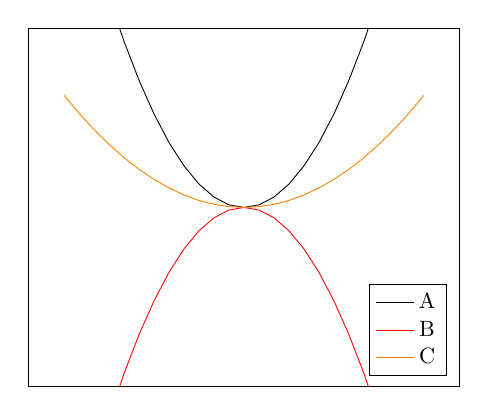
\begin{tikzpicture}[scale=0.8]
\begin{axis}[grid=none,
xmin=-3,xmax=3,
ymin=-3,ymax=3,
legend pos = south east,
xtick=\empty,
ytick=\empty,
minor tick={},
xlabel={}, ylabel={},
]
\addplot[domain=-2.5:2.5] {x^2};
\addlegendentry{A}
\addplot[domain=-2.5:2.5,red] {-x^2};
\addlegendentry{B}
\addplot[domain=-2.5:2.5,orange] {0.3*x^2};
\addlegendentry{C}
\end{axis}
\end{tikzpicture}
\end{center}
\end{exercise}

\begin{solution}
A is $y=x^4$; B is $y=-x^4$; C is $y=\frac{1}{4}^4$.
\end{solution}

\begin{exercise}
The area, $A$, of a unilateral triangle whose sides have length $a$ is given by:
\[
A=\frac{\sqrt{3}}{4}a^2
.\]
Find the side length $a$, in cm, which gives the area $A$ equal to $8 \text{ cm}^2$. Round off your answer to three decimal places.
\end{exercise}

\begin{solution}
4.298 cm
\end{solution}